\chapter{Introduction}\label{ch:introduction}

\vspace*{-50pt}

\begin{figure}[ht]
        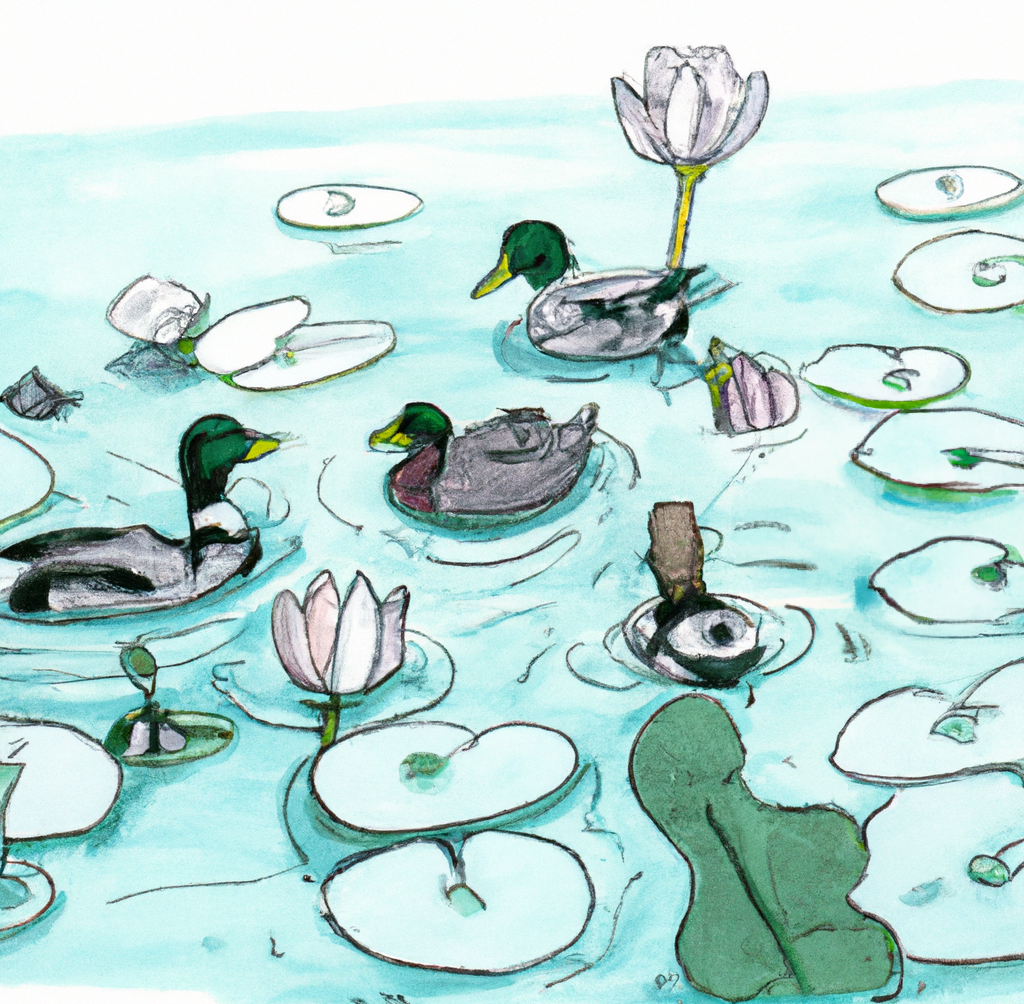
\includegraphics[width=0.35\textwidth, right]{img/dalle-ducks.png}
        \captionsetup{textformat=empty,labelformat=blank}
        \caption{Generated with Dall-E. \url{https://labs.openai.com/}. ``A duck dominating sitting on a sea rose''}
\end{figure}

\epigraph{\itshape Todo select another quote}{Lewis Caroll, \textit{XXXX}}

%\begin{wrapfigure}{R}{0.35\textwidth}
%\end{wrapfigure}

%\vspace*{25pt}

Quack! Quack! One second careless and suddenly, the dreaded \textit{geesiosi} clan conquered the Merganser Lake by claiming all the beautiful sea roses! 
% ducklings? Clan Name of thoses
Your befriended ducks want to gain it back and it seems that \textit{geesiosi} members are very afraid of your duck's quacking! If one of your ducks reclaims a sea rose, its voice will also rout all the neighboring geese!

Furthermore, we have to avoid that something like that never happens again. Therefore we have to hold the fort and protect against another rush of the \textit{geesiosi} by dwelling on the sea roses. 
This is very boring and, understandably, your brave ducks do not want to be alone and would like to have someone to quack with together!
Therefore, for every one of your brave ducks, there should be at least one other friend sitting one or two sea roses away.

The ducks have now asked for help and showed you a plan (see \cref{fig:duck-lake}) of the lake with all the sea roses marked in green. They want to know what the \textit{least} number of ducks is they have to send such that all the \textit{geesiosis} are put to flight - after all, they still have other things to do and do not want to send more ducks to fight than necessary!

% FROM https://creazilla.com/nodes/41547-duck-clipart
\begin{figure}
    \centering
    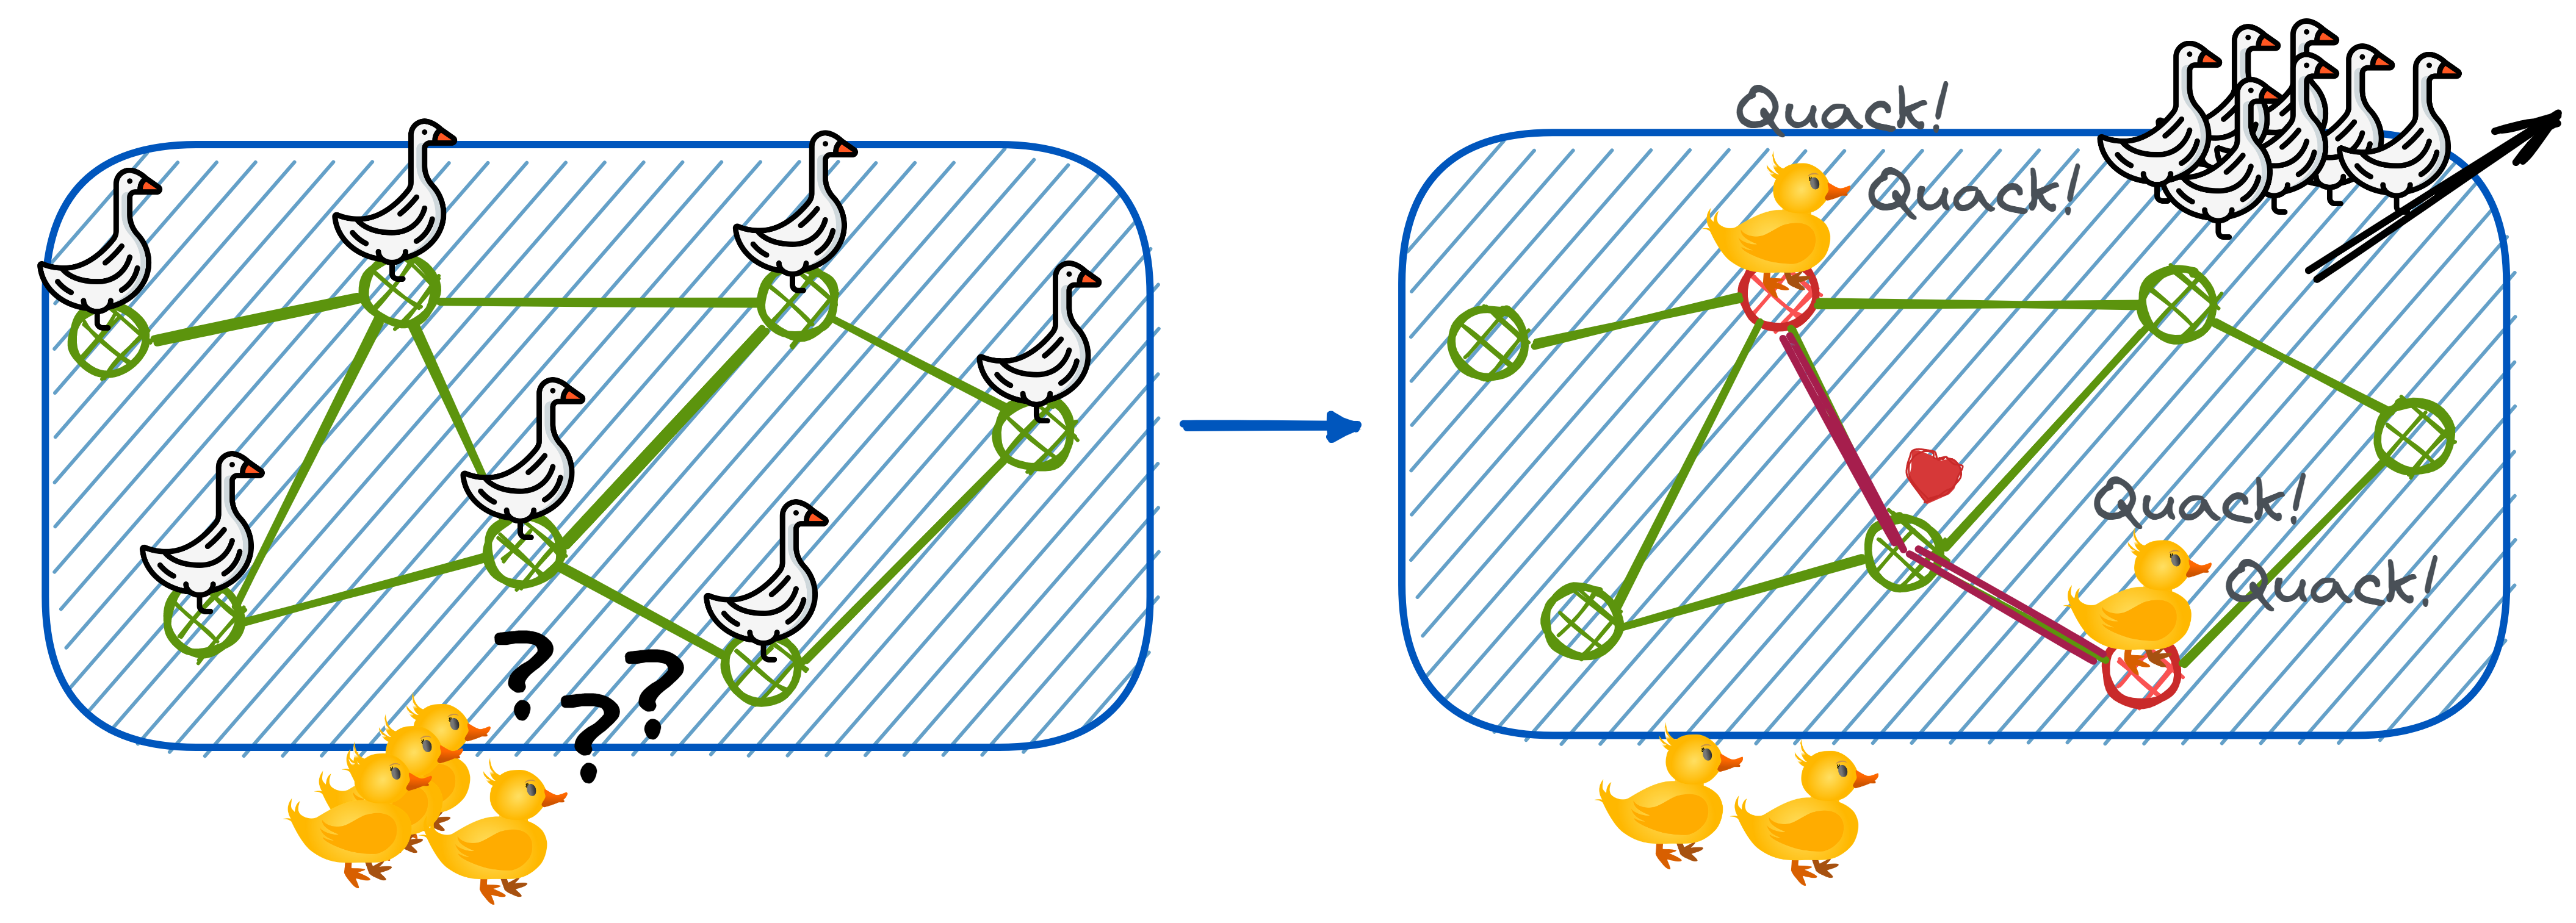
\includegraphics[width=0.9\columnwidth]{excalidraw/lake.png}
    \caption[Introductions: Merganser Lake. Own Drawing. Embedded icons under public domain from {\href{https://creazilla.com/}{https://creazilla.com/}}]{\textit{Only two ducks are needed to cover all sea roses.}}
    \label{fig:duck-lake}
\end{figure}

Can you help them? 


\textbf{Problem Definition}

\begin{prb}[DOMINATING SET {\cite[p. 586]{Cygan2015}}]{prb:ds}

    \begin{tabularx}{0.9\textwidth}{>{\hsize=0.30\hsize}X>{\hsize=0.8\hsize}X}
        \textbf{Input:} & Graph \G and an integer $k$\\
        \textbf{Question:} & Is there a set $X \subseteq V$ of size at most $k$ such that $N[X] = V$? \\
    \end{tabularx}
        
\end{prb}

\begin{prb}[SEMITOTAL DOMINATING SET {\cite{Goddard2014}}]{prb:tds}
    
    \begin{tabularx}{0.8\textwidth}{>{\hsize=0.35\hsize}X>{\hsize=0.8\hsize}X}
        \textbf{Input:} & Graph \G and an integer $k$\\
        \textbf{Question:} & Is there a subset $X \subseteq V$ of size at most $k$ such that $N[X] = V$ and for all $d_1 \in X$ there exists another $d_2 \in X$ such that $d(d_1, d_2) \leq 2$?\\
    \end{tabularx}
        
\end{prb}

\begin{prb}[TOTAL DOMINATING SET {\cite[p. 596]{Cygan2015}}]{prb:sds}
    
    \begin{tabularx}{0.8\textwidth}{>{\hsize=0.35\hsize}X>{\hsize=0.8\hsize}X}
        \textbf{Input:} & Graph \G and an integer $k$\\
        \textbf{Question:} & Does there exists a set $X \subseteq V$ of at most $k$ vertices of G such that for every $u \in V(G)$ there exists $v \in X$ with $\{u,v\} \in E$ \\
    \end{tabularx}
        
\end{prb}



\section{Content of the thesis}

In this thesis, we continue the systematic analysis of the \sdom problem by focusing on the parametrized complexity of the problem. 

Although the problem already had a lot of attention regarding classical complexity (CITE), only a few results are currently known for the parametrized variant. 

As far as we have seen, even the w-hardness of the general case has not been explicitly proven in the literature. 

In this thesis, we continue the journey toward a systematic analysis by stating some hardness results for specific graph classes for the problem.

\paragraph{Our contributions}
% TODO Better: 

Our main contributions consist of first showing the $w[2]$-hardness of \sdom for XXXX graphs.

\noindent As the \dom problem and the \tdom problem both admit a linear kernel for planar graphs, it is interesting to analyze whether these results also hold for the \sdom problem which lies in between these two. 
%TODO by relxing the witness of these two provlemsproblems.

Having these kernels also for other variants like \eddom, \efdom, \cdom, \rbdom lent us great confidence that the result will also work for \sdom on planar graphs.

%% TODO Find more  .

Following the approach from ... which already relies on the technique given in, we give some simple data reduction rules for \sdom on planar graphs leading to a linear kernel. More precisely, we are going to prove the following central theorem of this thesis:

With some modifications, we were able to transfer the approach given by Garnero and Sau in \cite{Garnero2018} to the \sdom problem.

\begin{restatable}[]{theorem}{centraltheo}\label{thm:central}
    The \sdom problem parametrized by solution size admits a linear kernel on planar graphs. There exists a polynomial-time algorithms that given a planar graph $(G, k)$, either correctly reports that $(G, k)$ is a NO-instance or returns an equivalent instance $(G', k)$ such that $\abs{V(G')} \leq \kernelsize \cdot k$.
\end{restatable}

\dom problem and \tdom problem, both already 

\begin{figure}[t]
     \begin{equation*}
         \tikzfig{fig/tikz/ds-examples}
     \end{equation*}
    \caption[An example for various dominating sets]{\textit{An example  for a \dom, \sdom and \tdom, where $\gamma(G) < \gamma_{2t}(G) < \gamma_t(G)$ are strict. In the first case, only two vertices suffice to dominate all others. In the second one, we need a witness between $d_1$ and $d_2$ that is at most distance two. In the last case, $d_1$ and $d_2$ both need a neighbor in the \tdom.}}
    \label{figd:dsexamples}
\end{figure}
